% !TeX program = pdflatex
\documentclass[10pt,a4paper]{article}
\usepackage[spanish,es-nodecimaldot,es-noshorthands]{babel}
\usepackage[T1]{fontenc}
\usepackage[utf8]{inputenc}
\usepackage{lmodern}
\renewcommand{\familydefault}{\sfdefault}
\usepackage[a4paper,left=1.55cm,right=1.55cm,top=1.3cm,bottom=1.45cm]{geometry}
\usepackage{graphicx}
\usepackage{xcolor}
\usepackage{booktabs}
\usepackage{hyperref}
\definecolor{cchenpurple}{HTML}{483888}
\setlength{\parindent}{0pt}
\setlength{\parskip}{4pt}
\begin{document}
{\Large\bfseries\color{cchenpurple} Resumen ejecutivo: fuentes implementadas desde matriz Fernanda}

Fecha: 2026-05-19

Se documentaron 22 fuentes implementadas provenientes de la matriz de Fernanda. El paquete separa conexiones directas/API, fuentes derivadas por semillas, runtime local y casos que requieren revision antes de presentarse como fuente estable.

\section*{Lectura ejecutiva}
\begin{itemize}
\item Fuentes directas/API listas: 12.
\item Fuentes derivadas o por semillas: 6.
\item Fuentes bloqueadas por token: 1.
\item Matches a revisar: 1.
\item Regla metodologica: no se descarga universo completo; toda fuente debe operar CCHEN-only o por semillas justificadas.
\end{itemize}

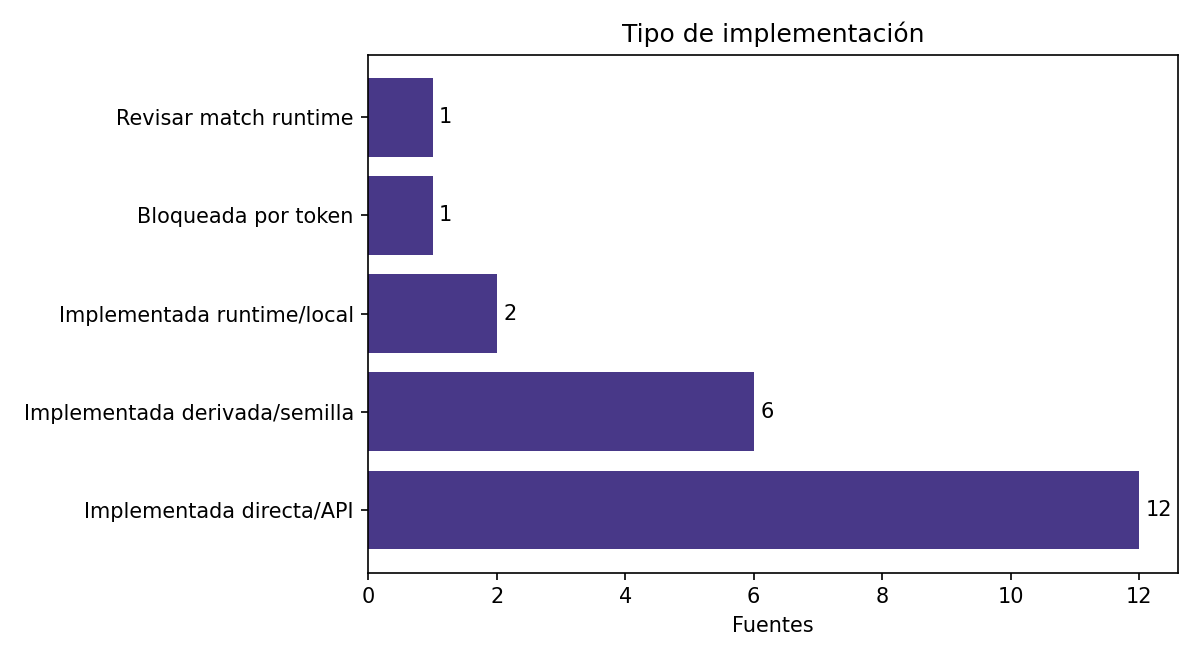
\includegraphics[width=\textwidth]{assets/tipo_implementacion_fuentes.png}

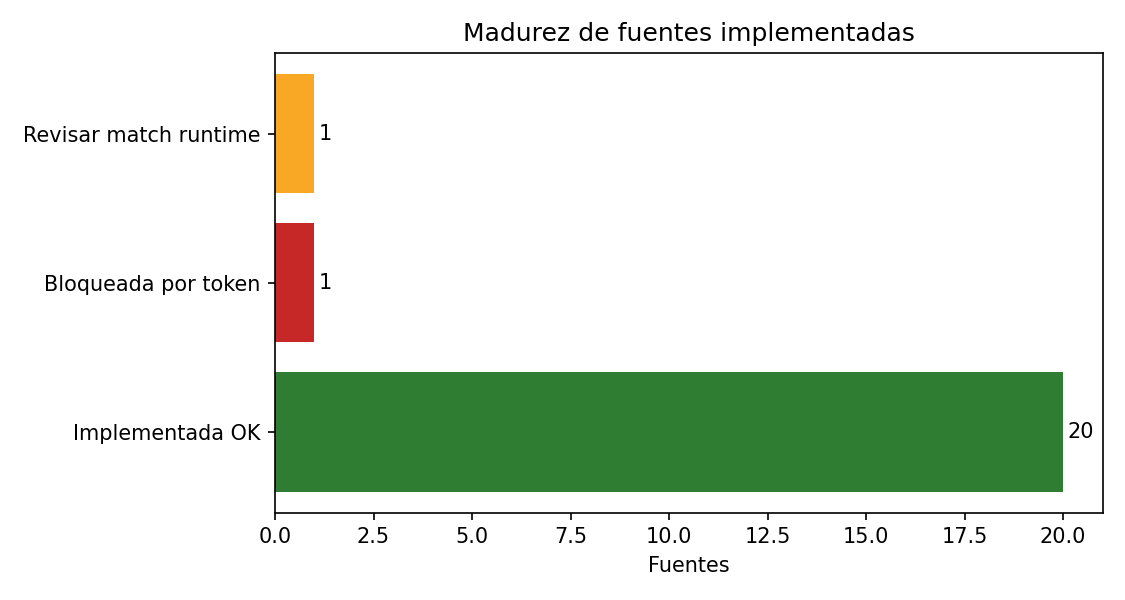
\includegraphics[width=\textwidth]{assets/madurez_fuentes_implementadas.png}

\section*{Decisiones operativas}
\begin{tabular}{lr}
\toprule
Decision & Fuentes \\
\midrule
mantener & 14 \\
mantener\_con\_observacion & 6 \\
bloqueada\_por\_token & 1 \\
revisar\_match & 1 \\
\bottomrule
\end{tabular}

\section*{Alertas para consultora}
\begin{itemize}
\item PatentsView / USPTO requiere \texttt{PATENTSVIEW\_API\_KEY}; no reemplaza INAPI local.
\item Google Finance / News monitor requiere revision: el runtime monitorea noticias CCHEN/nuclear, no datos financieros.
\item Las fuentes Life Sciences derivadas deben presentarse como evidencia por semillas hasta implementar extractores directos.
\item Los conteos multiples son artefactos distintos y no se suman como tabla unica.
\end{itemize}
\end{document}
